%%
% Final presentation — GD-2025 k-planarity solver project.
% Same TUM beamer template as main.tex (intermediate talk).
% Compile on Overleaf with the provided latexmkrc (TEXINPUTS -> tum/).
%%

\documentclass[
  english,
  aspectratio=169,
]{tumbeamer}

% load additional packages
\usepackage{booktabs}
\usepackage{tikz}
\usetikzlibrary{positioning,arrows.meta,calc}
\usepackage{pgfplots}\pgfplotsset{compat=1.18}
\definecolor{accent}{HTML}{2A7DB0}
\definecolor{warm}{HTML}{D85A30}
\definecolor{teal}{HTML}{0F8A6B}
\definecolor{muted}{HTML}{888780}

% presentation metadata
\title{Minimising \texorpdfstring{$k$}{k} in Straight-Line Graph Drawings}
\subtitle{Final Presentation -- Graph Drawing Contest k-planarity Solver}
\author{Amine \and Berkay \and Yi\u{g}it}

\institute{Chair for Efficient Algorithms (ALGO)\\Department of Computer Science\\Technical University of Munich}
\date[06/2026]{June 2026}

\footline{\insertauthor~|~\insertshorttitle~|~\insertshortdate}

\TUMbeamersetup{
  title page = TUM tower,
  part page = TUM toc,
  section page = TUM toc,
  content page = TUM more space,
  tower scale = 1.0,
  headline = TUM threeliner,
  footline = TUM default,
  headline on = {title page},
  footline on = {every page, title page=false},
}

\begin{document}

\maketitle

\begin{frame}{Outline}
  \tableofcontents
\end{frame}

% =====================================================================
%  Bölümler — 10-15 dk hedef: ~13 içerik slaytı.
%  journey.tex        : problem, başlangıç noktası, platform, zaman çizelgesi
%  what_we_built.tex  : engineering, k-critical, init hikâyeleri, ablation'lar
%  orchestrator.tex   : half-sharing, adaptive budget scheduler, deadline safety, UI
%  results_lessons.tex: final tablo, A8 grafiği, dersler, kalanlar
% =====================================================================
\section{The Problem \& Where We Started}


\iffalse
\begin{frame}{Our Journey}
  \textbf{Starting point:} a faithful re-implementation of the winning GD'25 entry
  (Bianchetti \& Moalic, \emph{LIPIcs.GD.2025.43}).
  \begin{itemize}
    \item Two-phase Simulated Annealing: phase 1 minimises $\chi$, phase 2 minimises $k$
          with a dual fitness ($\Delta K_{\text{local}}$ first, $\Delta\chi$ as tie-break).
    \item C++17, zero dependencies; incremental crossing bookkeeping per move.
    \item Added our own method family on top: greedy \textbf{LNS}, \textbf{staged}
          (LNS $\to$ SA warm-start), \textbf{ILS} (SA rounds + random kicks).
  \end{itemize}
  \medskip
  \textbf{The state of the world in early June:}
  \begin{itemize}
    \item Automatic-8 produced \alert{invalid output} (vertex-on-edge overlaps survived repair)
          --- no file written at all.
    \item $\sim$12 minutes of setup before the solver even started on A8, final $k\approx 10\,000$.
    \item Per-move validity checks were $O(n\cdot\deg)$ --- the move loop \emph{is} the budget.
  \end{itemize}
\end{frame}

\begin{frame}{Our Experiment Platform (built early, paid off daily)}
  Every claim in this talk is reproducible because every run goes through one pipeline:
  \begin{itemize}
    \item \texttt{run\_contest.py} --- method registry, per-run directories, best-ever
          tracking per graph$\times$method, accumulated history.
    \item \textbf{Multi-worker portfolio}: same budget split across 4--8 seeds in parallel,
          report the best --- single-seed variance is huge (more on that later).
    \item Live web control panel (\texttt{server.py}): configure, start, stop runs;
          status table refreshes every 5\,s; Chart.js convergence plots.
    \item 219-graph external benchmark (\texttt{gda-testing}) for generalisation checks.
  \end{itemize}
  \medskip
  \textbf{Why it matters:} the decisive experiments of this project were cheap
  \emph{because} starting a controlled A/B took one command.
\end{frame}
\fi

\begin{frame}{The Journey at a Glance}
  \centering
  \resizebox{0.97\linewidth}{!}{%
  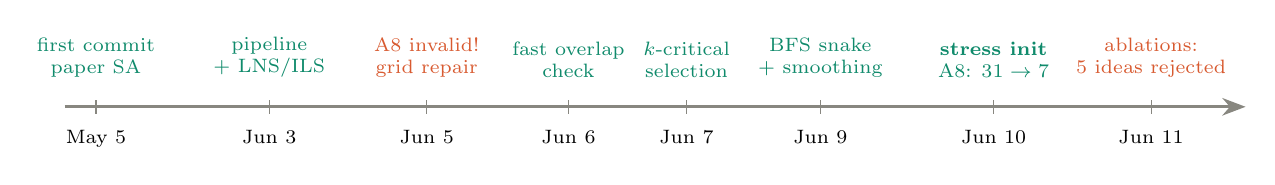
\begin{tikzpicture}[
      ev/.style={font=\scriptsize,align=center},
      good/.style={ev,text=teal},
      bad/.style={ev,text=warm}]
    \draw[muted,line width=1.2pt,-{Stealth}] (0,0) -- (15.0,0);
    \foreach \x/\d in {0.4/{May 5},2.6/{Jun 3},4.6/{Jun 5},6.4/{Jun 6},7.9/{Jun 7},9.6/{Jun 9},11.8/{Jun 10},13.8/{Jun 11}}
      {\draw[muted] (\x,-0.09) -- (\x,0.09); \node[ev,anchor=north] at (\x,-0.18){\d};}
    \node[good,anchor=south] at (0.4,0.25){first commit\\paper SA};
    \node[good,anchor=south] at (2.6,0.25){pipeline\\+ LNS/ILS};
    \node[bad,anchor=south]  at (4.6,0.25){A8 invalid!\\grid repair};
    \node[good,anchor=south] at (6.4,0.25){fast overlap\\check};
    \node[good,anchor=south] at (7.9,0.25){$k$-critical\\selection};
    \node[good,anchor=south] at (9.6,0.25){BFS snake\\+ smoothing};
    \node[good,anchor=south] at (11.8,0.25){\textbf{stress init}\\A8: $31\to 7$};
    \node[bad,anchor=south]  at (13.8,0.25){ablations:\\5 ideas rejected};
  \end{tikzpicture}}
  \medskip

  \begin{itemize}
    \item Three kinds of progress: \textcolor{teal}{\textbf{correctness}} (validity, repair),
          \textcolor{teal}{\textbf{throughput}} (grids, restart cost),
          \textcolor{teal}{\textbf{starting point}} (constructive + force-directed inits).
    \item And one kind of insight: \textcolor{warm}{\textbf{documented negative results}} ---
          knowing what \emph{doesn't} work and why.
  \end{itemize}
\end{frame}

\section{The Methods}

\begin{comment}
    

\begin{frame}{One Engine, Five Methods}
  \textbf{Shared core:} every method runs on the same incremental machinery ---
  per-move crossing deltas, spatial grids for candidate lookup, strict validity
  (no vertex on a foreign edge), and best-snapshot bookkeeping.
  \medskip
  \begin{center}
    \footnotesize
    \begin{tabular}{llll}
      \toprule
      \textbf{Method} & \textbf{Pipeline} & \textbf{Escapes local optima by} & \textbf{Binary} \\
      \midrule
      \texttt{sa}        & two-phase SA                    & temperature waves            & \texttt{sakgd} \\
      \texttt{sa-stress} & \textbf{stress init} $\to$ SA   & better start + waves         & \texttt{sfdp} + \texttt{sakgd} \\
      \texttt{staged}    & LNS (30\%) $\to$ SA (70\%)      & SA stage after greedy LNS    & \texttt{approach1} \\
      \texttt{staged-adaptive} & adaptive-LNS $\to$ SA     & growing neighbourhoods       & \texttt{approach1} \\
      \texttt{ils}       & SA rounds + random kicks        & perturbation between rounds  & \texttt{approach1} \\
      \bottomrule
    \end{tabular}
  \end{center}
  \medskip
  \textbf{Two-phase SA} (after the winning GD'25 entry):
  phase 1 minimises total crossings $\chi$ (untangles the drawing),
  phase 2 minimises the bottleneck $k$ with a dual fitness:
  $\Delta E = \Delta K_{\text{local}}$ if a touched edge's $k$ changes,
  else $\Delta\chi/\chi$ as a tiny tie-break.
\end{frame}

\end{comment}

\begin{frame}{Inside the SA Loop: Moves, Waves, Snapshots}
  \begin{columns}[T]
    \begin{column}{0.52\textwidth}
      \textbf{One move:}
      \begin{enumerate}
        \item pick a vertex --- crossing-weighted; in phase 2, biased to
              \emph{$k$-critical} endpoints,
        \item propose a position (Gaussian around current; radius shrinks
              with temperature),
        \item reject if occupied or vertex-on-edge,
        \item Metropolis: accept if $\Delta E\le 0$, else with
              probability $e^{-\Delta E/T}$.
      \end{enumerate}
      \medskip
      \textbf{Temperature waves:} inner loop cools $T$ per move;
      the outer loop restarts each wave from the best-so-far solution
      at a slightly lower starting temperature.
    \end{column}
    \begin{column}{0.45\textwidth}
      \textbf{Best-snapshot bookkeeping:}
      \begin{itemize}
        \item \texttt{saveBest()} --- whenever $(k,\chi)$ improves, copy the
              positions into \texttt{bestPos} (three fields, \emph{in RAM}).
        \item \texttt{restoreBest()} --- copy \texttt{bestPos} back and rebuild
              the tables: at wave ends, and once more before writing output.
      \end{itemize}
      \medskip
      \textbf{Stateless by design:} no files, no caches, nothing survives the
      process. Two runs on the same input are fully independent ---
      warm-starting across runs exists only as an explicit, off-by-default
      pipeline flag.
    \end{column}
  \end{columns}
\end{frame}

\begin{frame}{Method Shoot-Out: Same Seeds, Same Budgets}
  All five methods, all nine instances, one controlled sweep
  (4 workers, seeds 42--45, budgets 2/4/6\,min by size; best $k$ of 4 workers; all outputs validated):
  \begin{center}
    \footnotesize
    \begin{tabular}{lrrrrr}
      \toprule
      \textbf{Graph} & \texttt{sa} & \texttt{sa-stress} & \texttt{ils} & \texttt{staged} & \texttt{st.-adaptive} \\
      \midrule
      Automatic-1 & \textbf{9}  & \textbf{9}  & \textbf{9}  & \textbf{9}  & \textbf{9}  \\
      Automatic-2 & 4           & 4           & \textbf{3}  & \textbf{3}  & \textbf{3}  \\
      Automatic-3 & \textbf{35} & 37          & 37          & 37          & 37          \\
      Automatic-4 & 7           & \textbf{6}  & 7           & 7           & 7           \\
      Automatic-5 & 77          & \textbf{75} & 79          & 78          & 78          \\
      Automatic-6 & \textbf{669}& 737         & 787         & 754         & 765         \\
      Automatic-7 & 50          & \textbf{29} & 57          & 52          & 53          \\
      Automatic-8 & 47          & \textbf{8}  & 309         & 52          & 48          \\
      Automatic-9 & 57          & \textbf{11} & 53          & 59          & 56          \\
      \bottomrule
    \end{tabular}
  \end{center}
  \smallskip
  \begin{itemize}
    \item \texttt{sa-stress} wins or ties \textbf{6 of 9} --- and by $2$--$6\times$ where
          the canvas is tight (A7/A8/A9).
    \item Dense A6 is the exception: plain \texttt{sa} wins; stress init actively hurts there.
  \end{itemize}
\end{frame}

% --- slide 1 of 2: numbers ---
\begin{frame}{Staged-Adaptive \& ILS: The Numbers (A7--A9)}
  \texttt{sa-stress} vs.\ the two alternatives on the three hardest instances
  (4 workers, seeds 42--45, equal budgets; best $k$ of 4 workers):
  \bigskip
  \begin{center}
    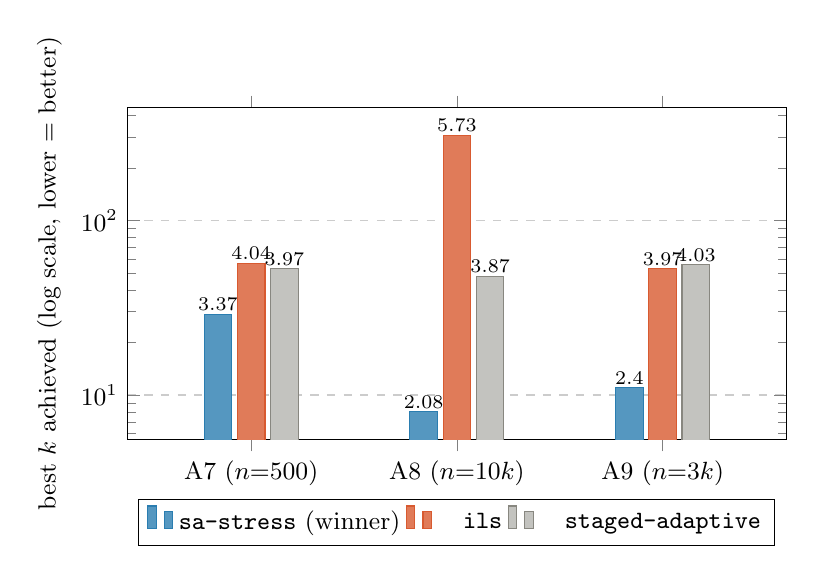
\begin{tikzpicture}
      \begin{axis}[
        ybar, bar width=10pt,
        ymode=log,
        ylabel={best $k$ achieved (log scale, lower = better)},
        symbolic x coords={A7,A8,A9},
        xtick=data,
        xticklabels={A7 ($n{=}500$), A8 ($n{=}10\text{k}$), A9 ($n{=}3\text{k}$)},
        legend style={at={(0.5,-0.18)}, anchor=north, legend columns=3, font=\small},
        width=0.82\textwidth, height=5.8cm,
        ymajorgrids=true, grid style={dashed, gray!40},
        every axis/.append style={font=\small},
        nodes near coords,
        nodes near coords style={font=\scriptsize, inner sep=1pt},
        enlarge x limits=0.3,
      ]
        \addplot[fill=accent!80, draw=accent] coordinates {(A7,29) (A8,8)   (A9,11)};
        \addplot[fill=warm!80,   draw=warm]   coordinates {(A7,57) (A8,309) (A9,53)};
        \addplot[fill=muted!50,  draw=muted]  coordinates {(A7,53) (A8,48)  (A9,56)};
        \legend{\texttt{sa-stress} (winner),\quad\texttt{ils},\quad\texttt{staged-adaptive}}
      \end{axis}
    \end{tikzpicture}
  \end{center}
  \smallskip
  \textbf{A8 gap: $38\times$} --- \texttt{ils} reaches $k=309$, \texttt{sa-stress} reaches $k=8$.
\end{frame}

% --- slide 2 of 2: why ---
\begin{frame}{Staged-Adaptive \& ILS: Why They Lose}
  \begin{columns}[T]
    \begin{column}{0.48\textwidth}
      \textbf{ILS} (SA rounds $+$ random kicks)
      \medskip

      \begin{center}
      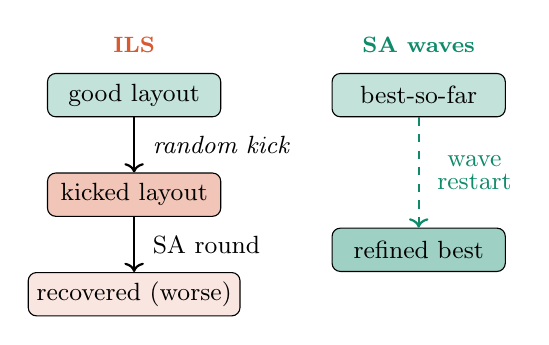
\begin{tikzpicture}[font=\small, node distance=0.7cm and 0.8cm,
          box/.style={draw, rounded corners=3pt, minimum width=2.2cm,
                      minimum height=0.55cm, align=center, inner sep=3pt}]
        \node[box, fill=teal!25]              (g)  {good layout};
        \node[box, fill=warm!35,  below=of g] (k)  {kicked layout};
        \node[box, fill=warm!15,  below=of k] (r)  {recovered (worse)};
        \draw[->, thick] (g) -- node[right=3pt]{\textit{random kick}} (k);
        \draw[->, thick] (k) -- node[right=3pt]{SA round} (r);

        \node[box, fill=teal!25, right=1.4cm of g]  (b1) {best-so-far};
        \node[box, fill=teal!40, below=1.4cm of b1] (b2) {refined best};
        \draw[->, thick, dashed, color=teal]
          (b1) -- node[right=3pt]{\shortstack{wave\\restart}} (b2);

        \node[above=4pt of g,  font=\footnotesize\bfseries, text=warm] {ILS};
        \node[above=4pt of b1, font=\footnotesize\bfseries, text=teal] {SA waves};
      \end{tikzpicture}
      \end{center}

      \smallskip
      On A8, untangling takes the whole budget.
      One kick resets that work.
      Waves restart \emph{from the best} --- no destruction.
    \end{column}
    \begin{column}{0.48\textwidth}
      \textbf{Staged-adaptive} (adaptive LNS $\to$ SA)
      \medskip
      \begin{itemize}
        \item LNS displaces many vertices at once, ignoring crossing geometry.
        \item The growing neighbourhood adds overhead, not quality.
        \item SA starts \emph{later} from a layout no better than stress init
              provides for free in seconds.
      \end{itemize}
      \vfill
      \textbf{Both dropped.}
      The complexity (LNS infrastructure, kick logic) adds nothing.
      \texttt{sa-stress} dominates on every large instance.
      The real lever was always the \emph{starting point}.
    \end{column}
  \end{columns}
\end{frame}

\section{Visual Demo}

\begin{frame}{Automatic-7 — Example Run (\texttt{sa-stress}, 3\,min)}
  \small Automatic-7: $n=500$, $m=1\,740$, canvas $115{\times}116$.
  \medskip
  \begin{columns}[c]
    \begin{column}{0.47\textwidth}
      \centering
      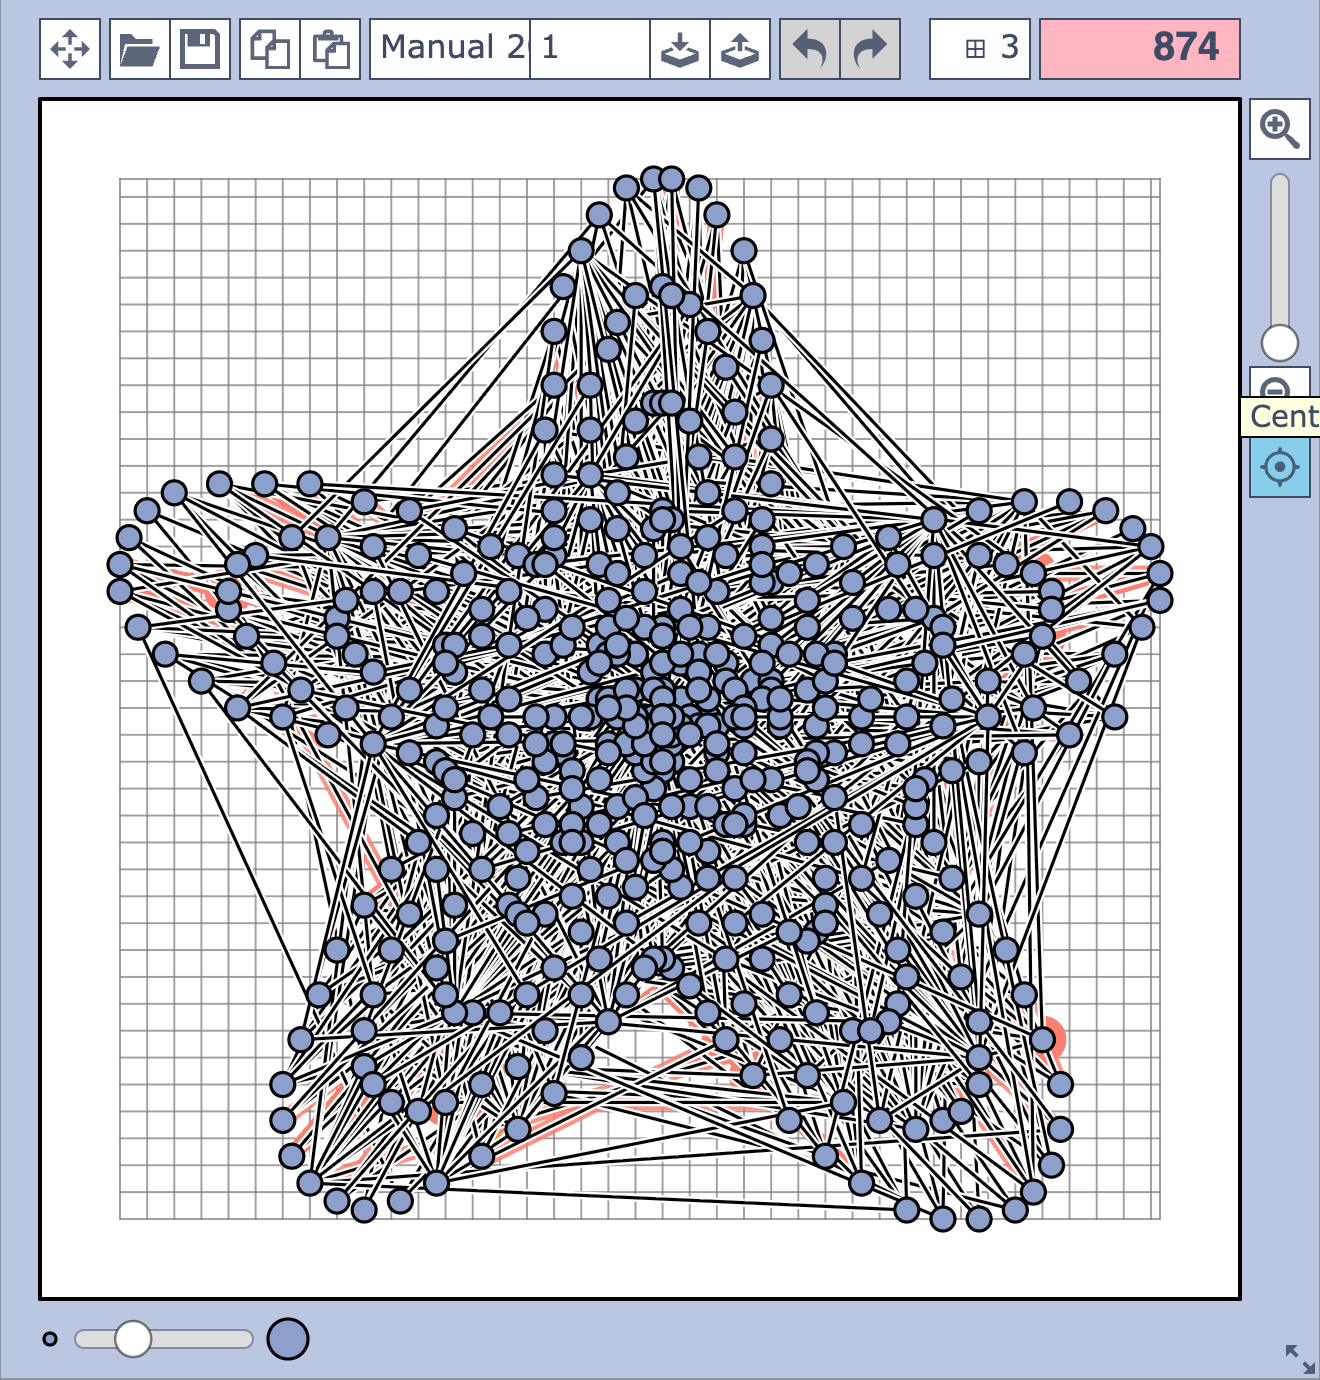
\includegraphics[width=\textwidth]{img/A7_0_original.png}\\[2pt]
      \textbf{Original} \quad $k = 858$
    \end{column}
    \begin{column}{0.47\textwidth}
      \centering
      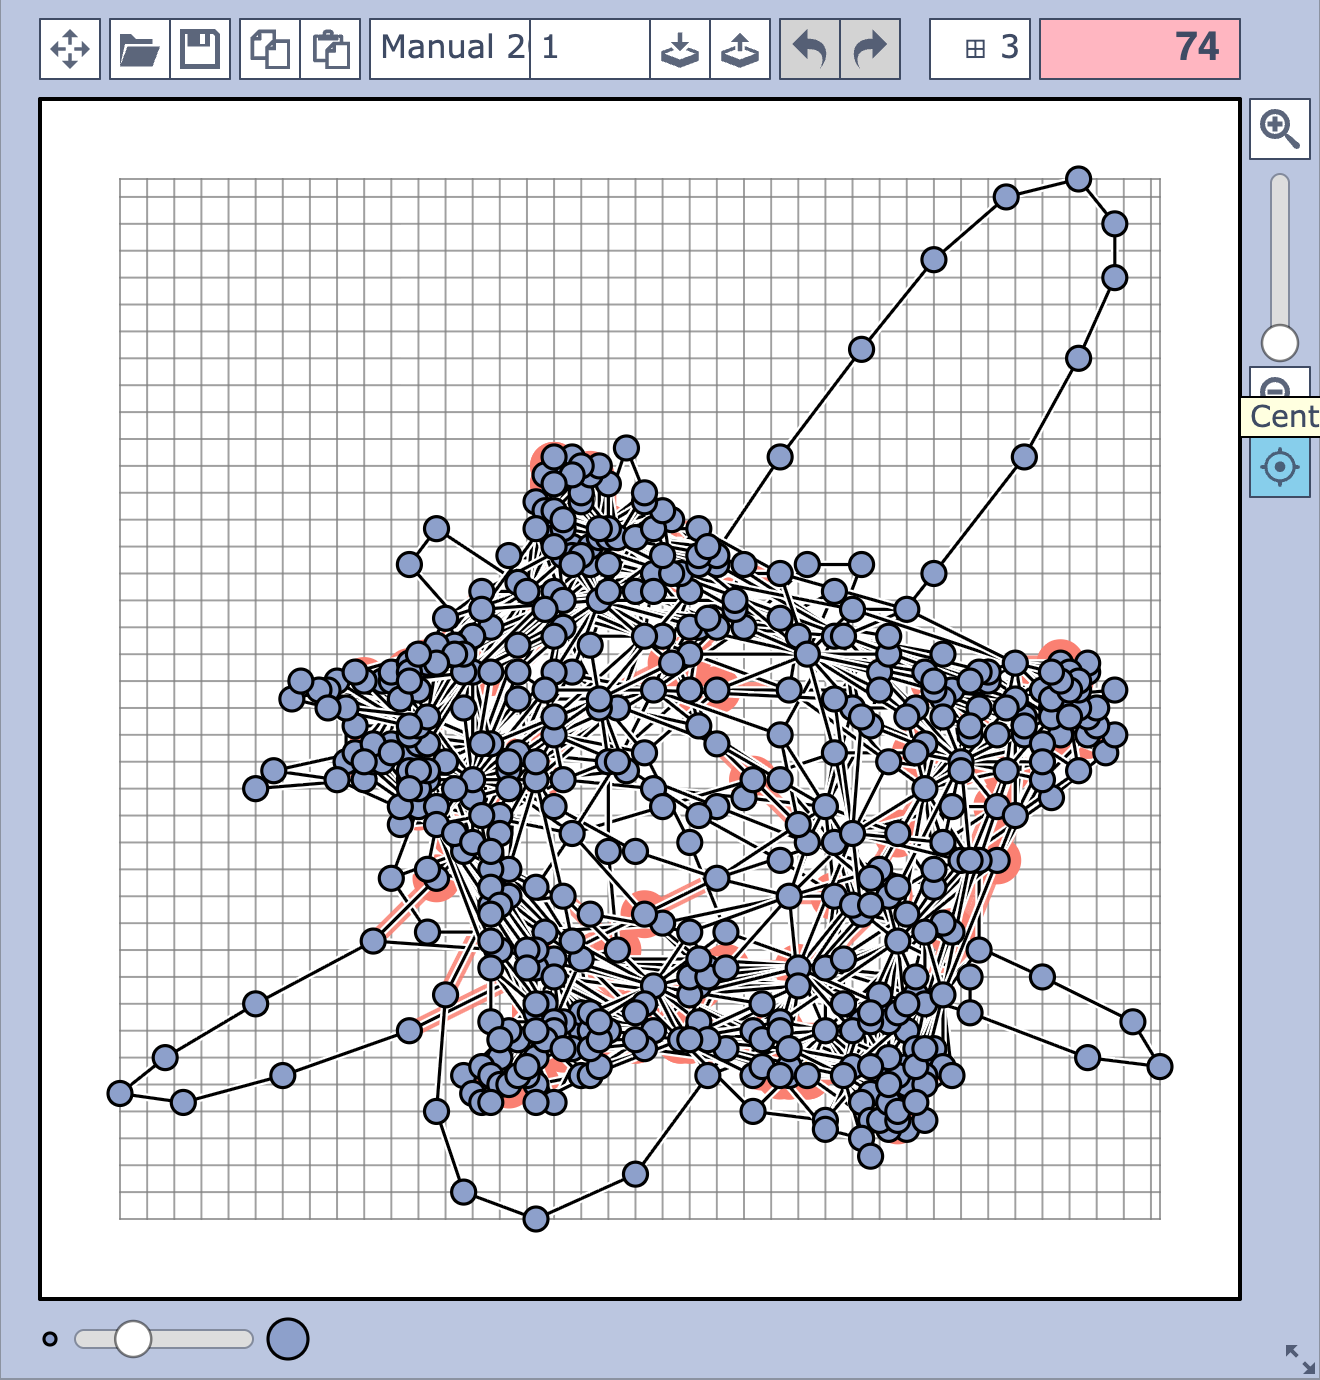
\includegraphics[width=\textwidth]{img/A7_1_stress.png}\\[2pt]
      \textbf{Stress Init} (sfdp) \quad $k = 74$
    \end{column}
  \end{columns}
\end{frame}

\begin{frame}{Automatic-7 — Example Run (\texttt{sa-stress}, 3\,min)}
  \small Automatic-7: $n=500$, $m=1\,740$, canvas $115{\times}116$.
  \medskip
  \begin{columns}[c]
    \begin{column}{0.47\textwidth}
      \centering
      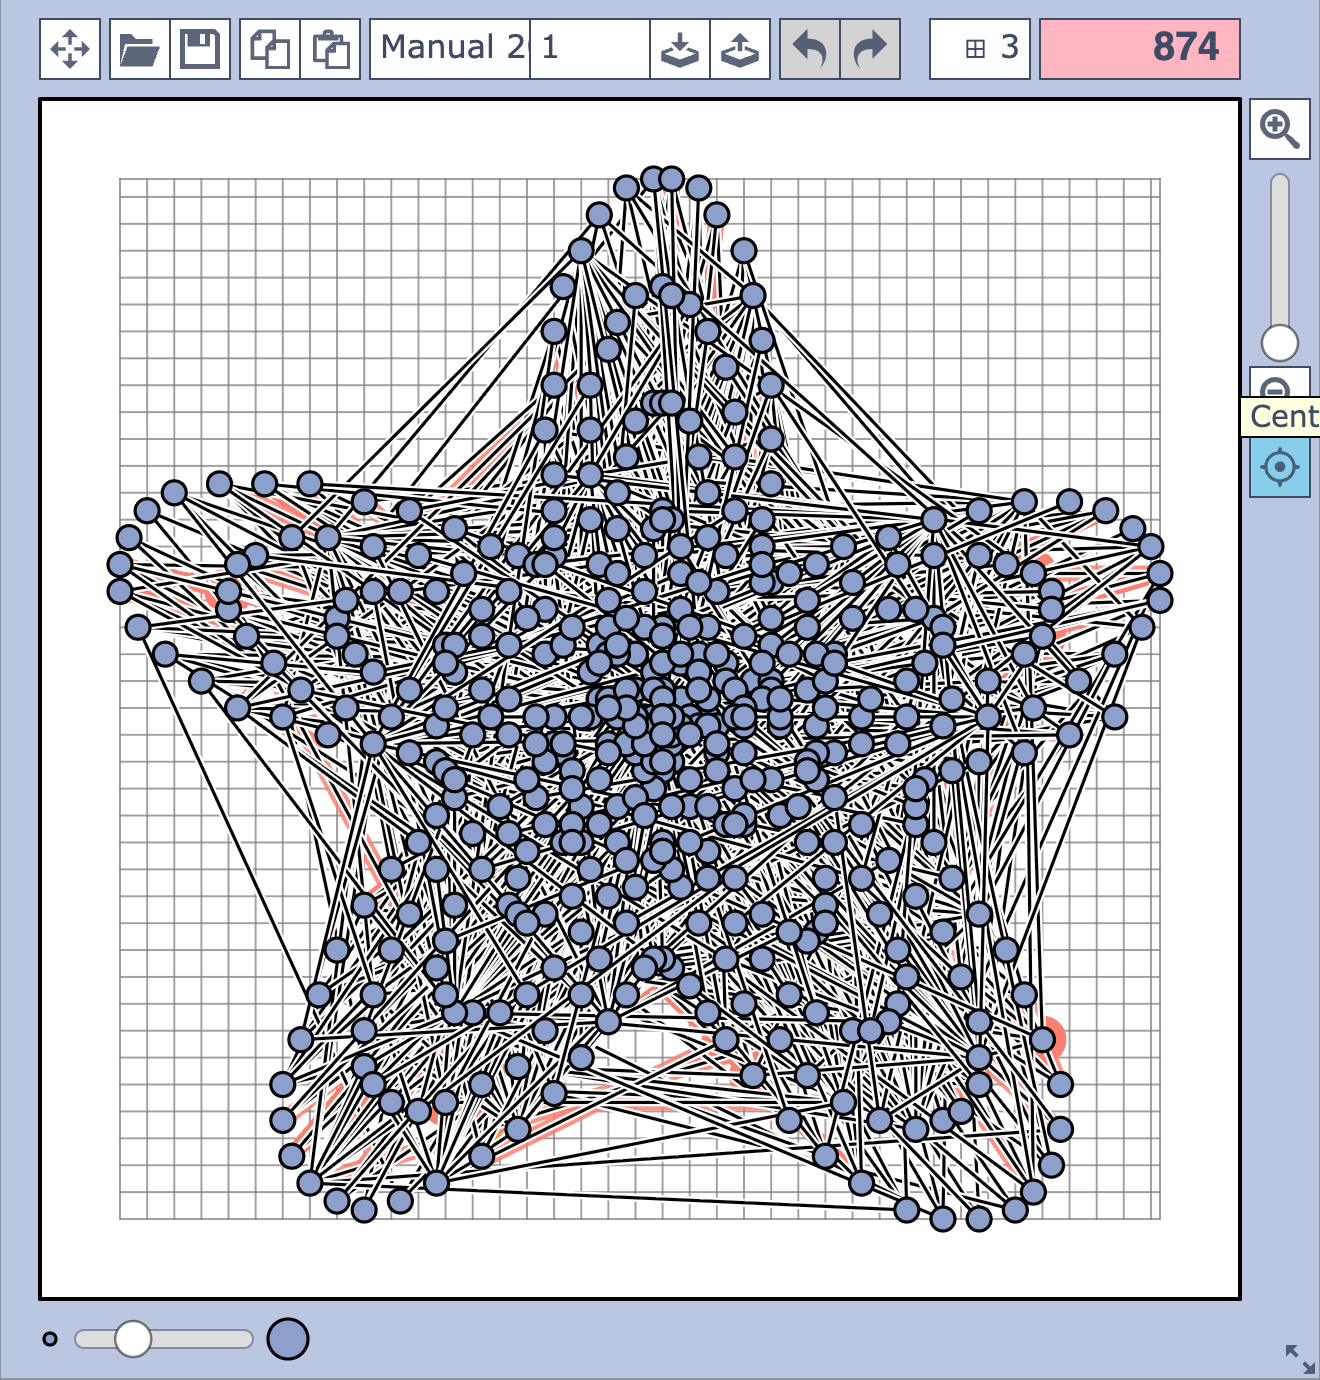
\includegraphics[width=\textwidth]{img/A7_0_original.png}\\[2pt]
      \textbf{Original} \quad $k = 858$
    \end{column}
    \begin{column}{0.47\textwidth}
      \centering
      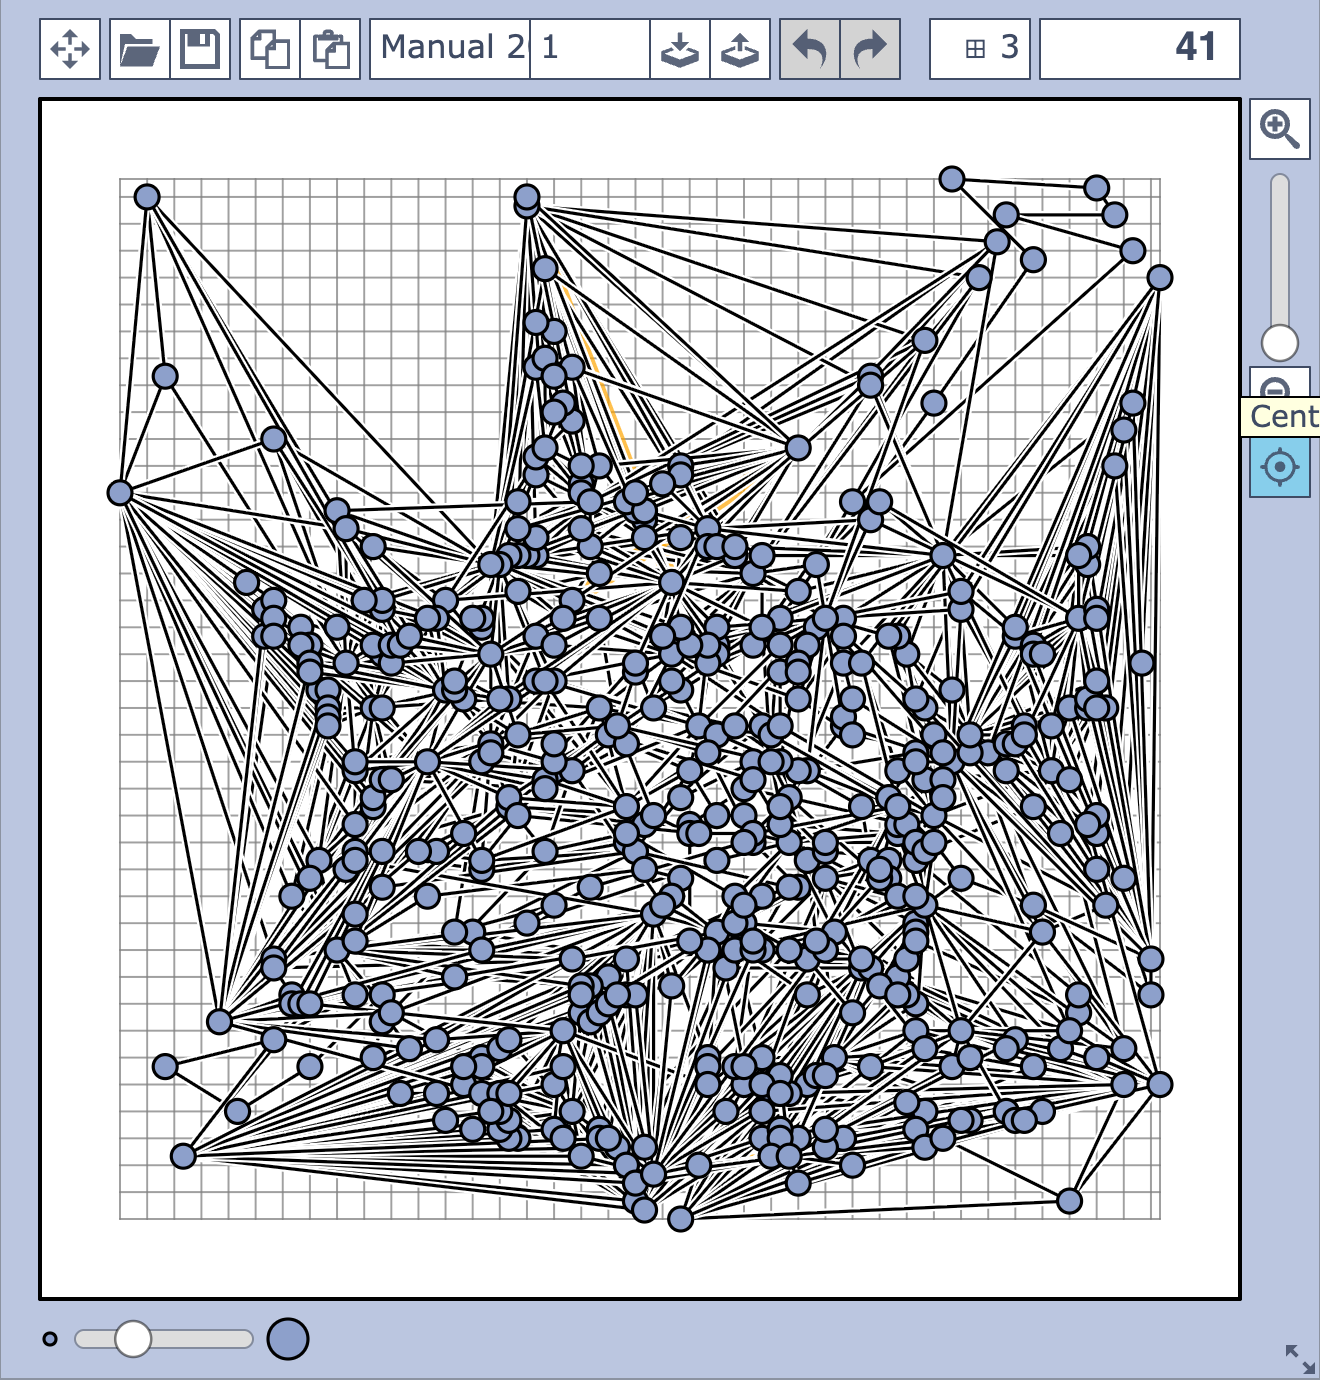
\includegraphics[width=\textwidth]{img/A7_2_phase1.png}\\[2pt]
      \textbf{Phase 1} — minimise $\chi$ \quad $k = 41$
    \end{column}
  \end{columns}
\end{frame}

\begin{frame}{Automatic-7 — Example Run (\texttt{sa-stress}, 3\,min)}
  \small Automatic-7: $n=500$, $m=1\,740$, canvas $115{\times}116$.
  \medskip
  \begin{columns}[c]
    \begin{column}{0.47\textwidth}
      \centering
      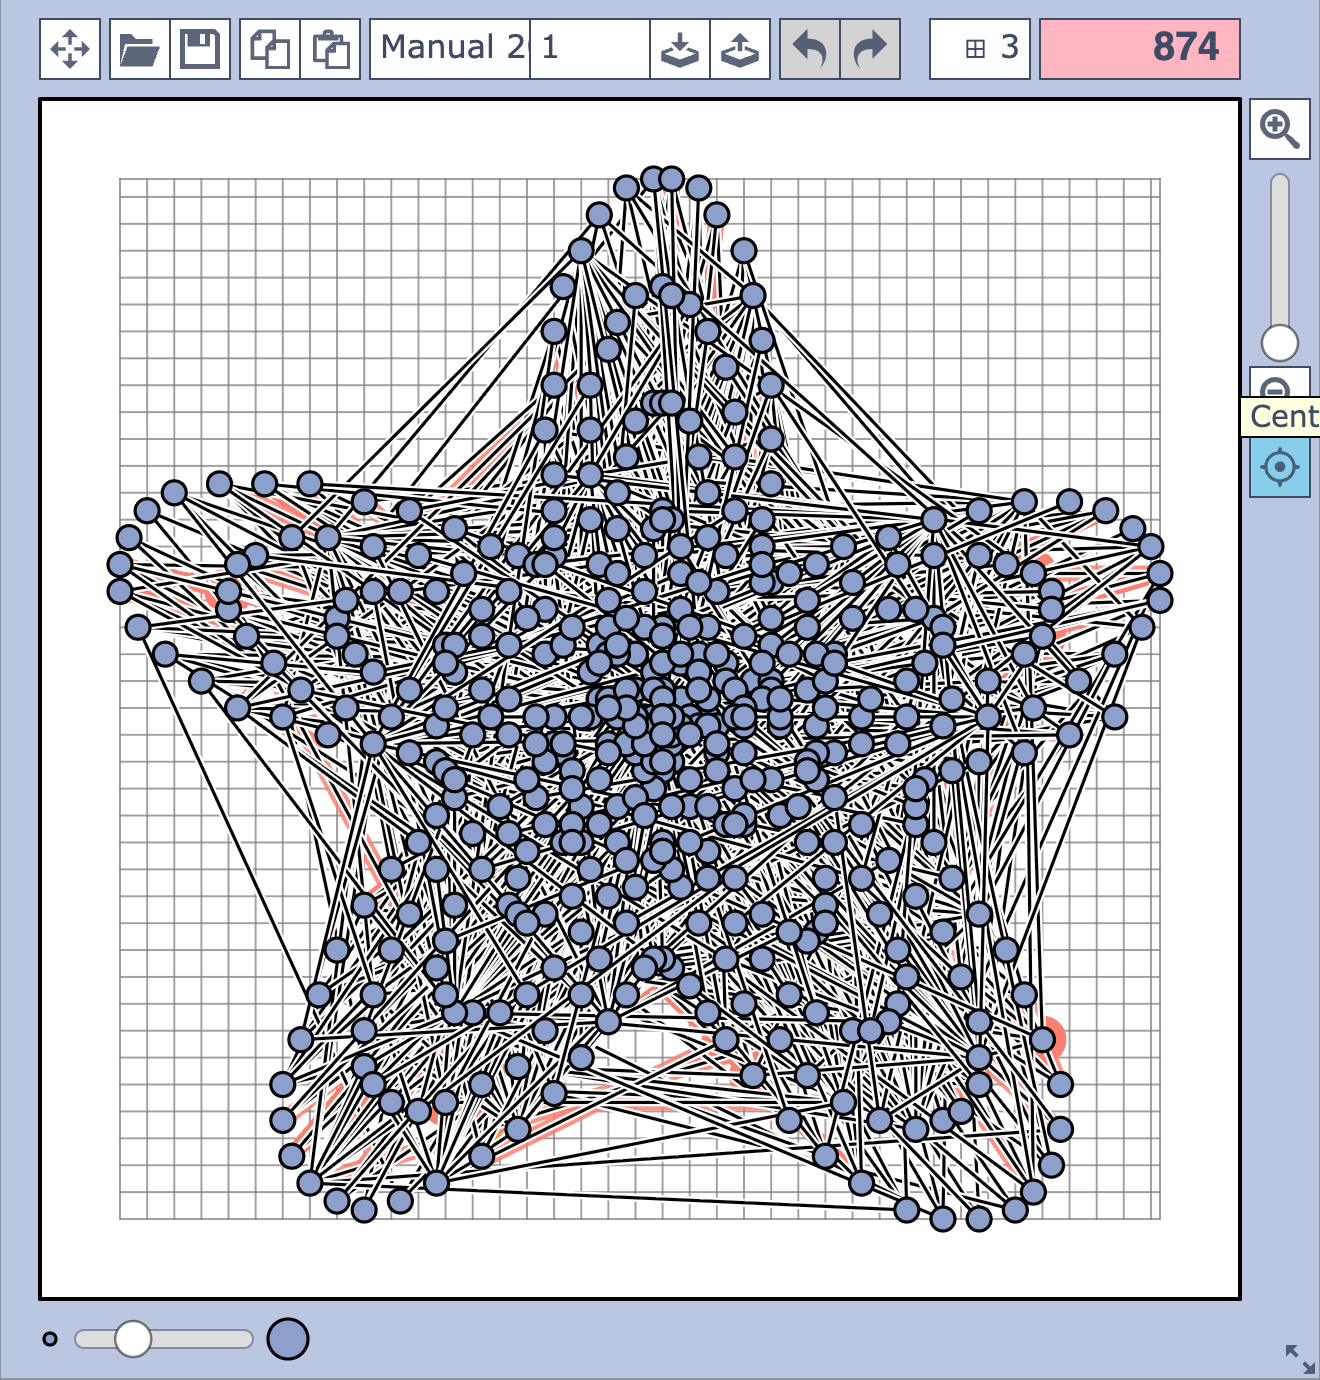
\includegraphics[width=\textwidth]{img/A7_0_original.png}\\[2pt]
      \textbf{Original} \quad $k = 858$
    \end{column}
    \begin{column}{0.47\textwidth}
      \centering
      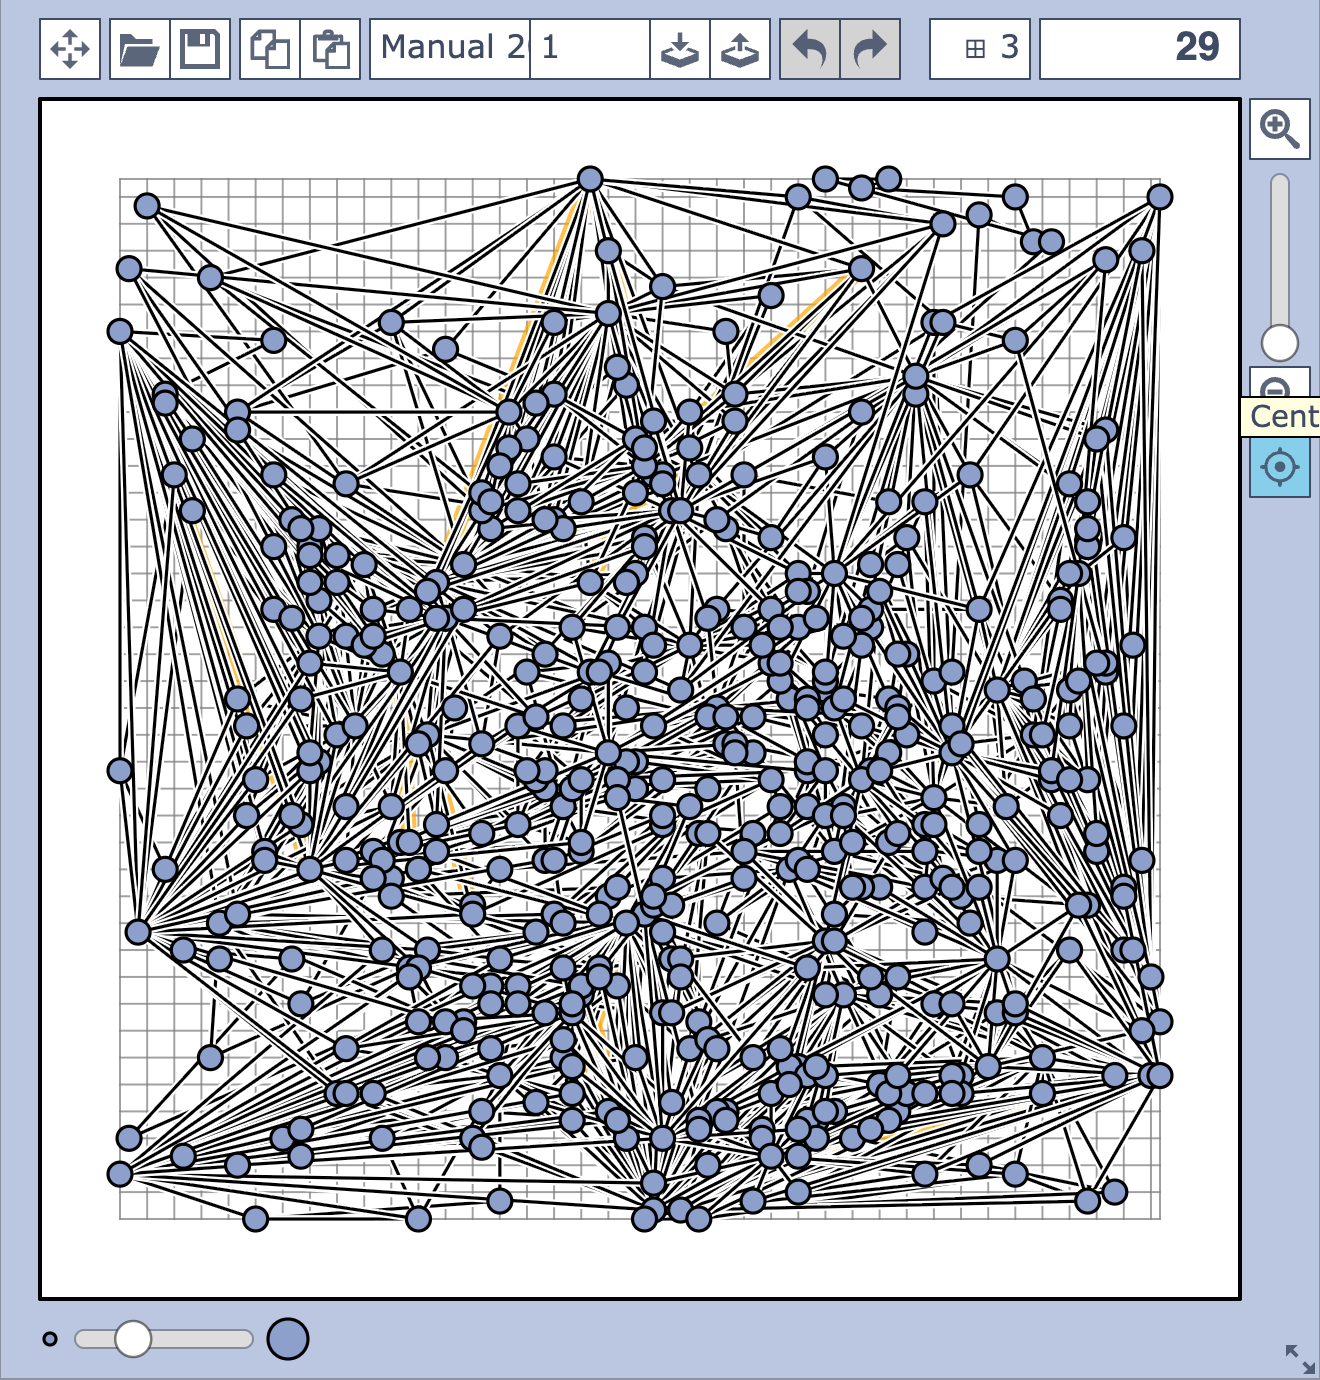
\includegraphics[width=\textwidth]{img/A7_3_phase2.png}\\[2pt]
      \textbf{Phase 2} — minimise $k$ \quad $k = 29$
    \end{column}
  \end{columns}
\end{frame}

\begin{frame}{Automatic-7 — All Stages at a Glance}
  \begin{columns}[c]
    \begin{column}{0.23\textwidth}
      \centering
      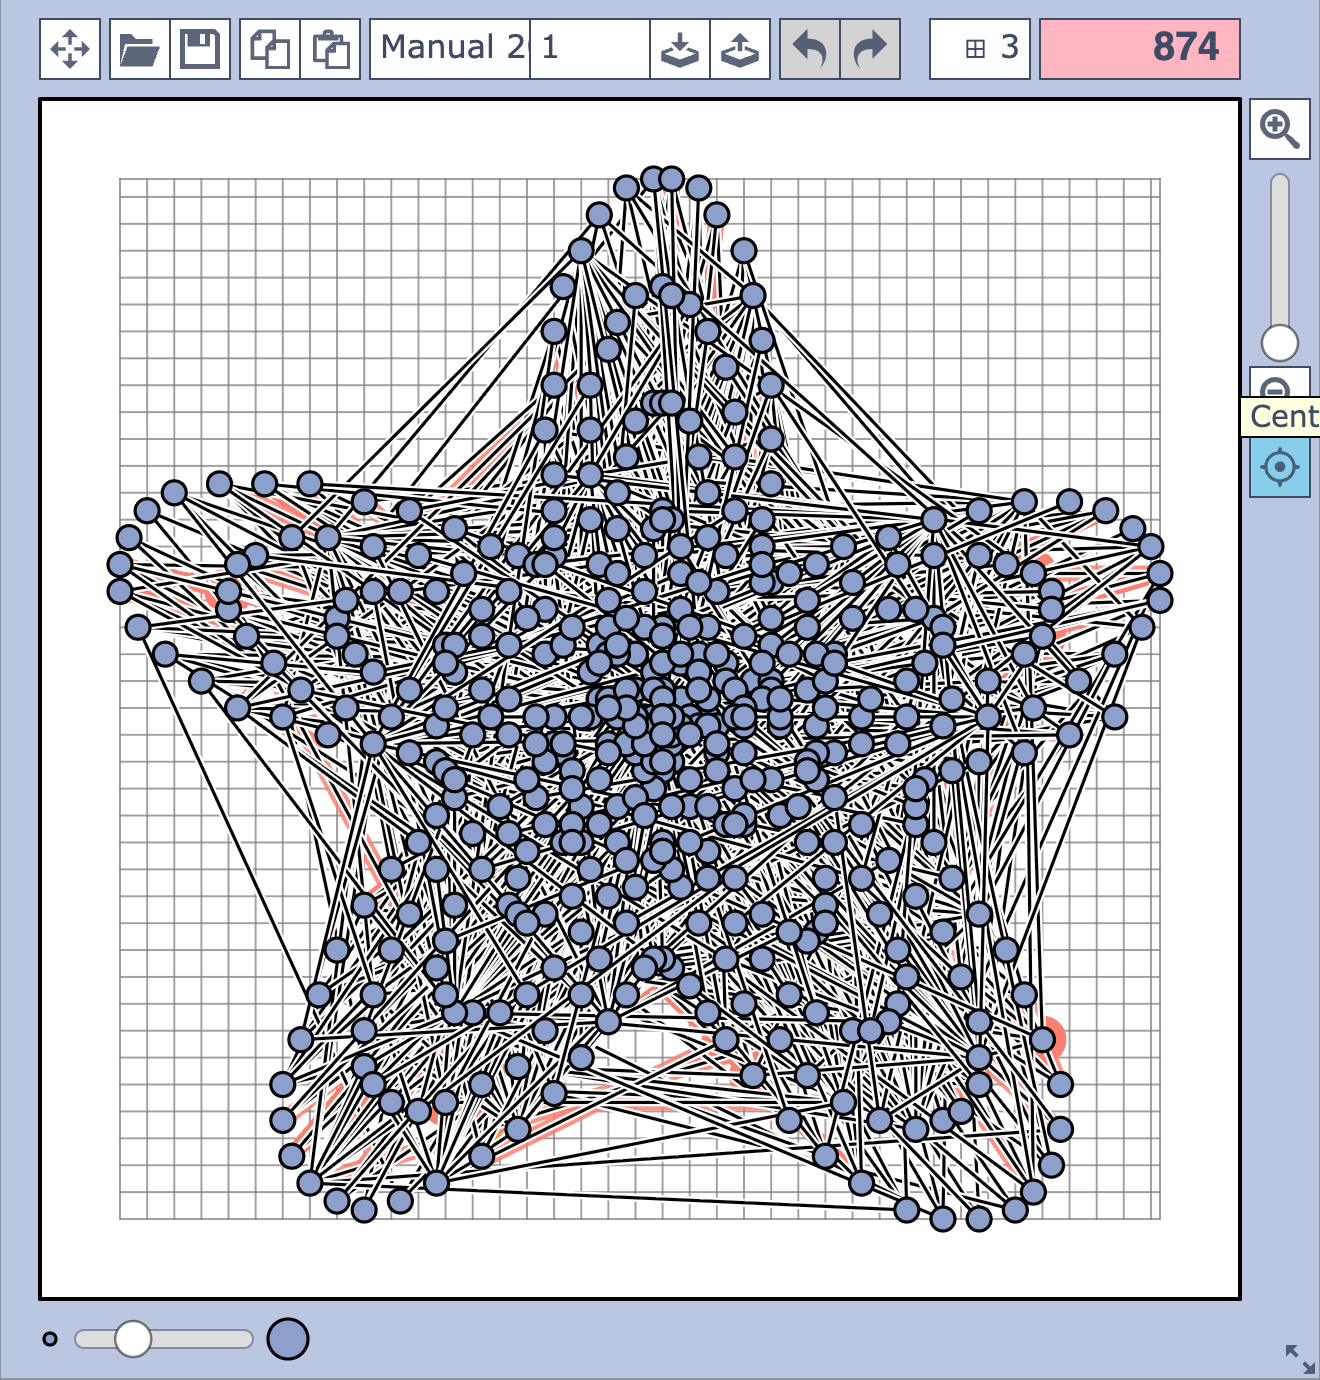
\includegraphics[width=\textwidth]{img/A7_0_original.png}\\[2pt]
      \footnotesize\textbf{Original}\\$k=858$
    \end{column}
    \begin{column}{0.23\textwidth}
      \centering
      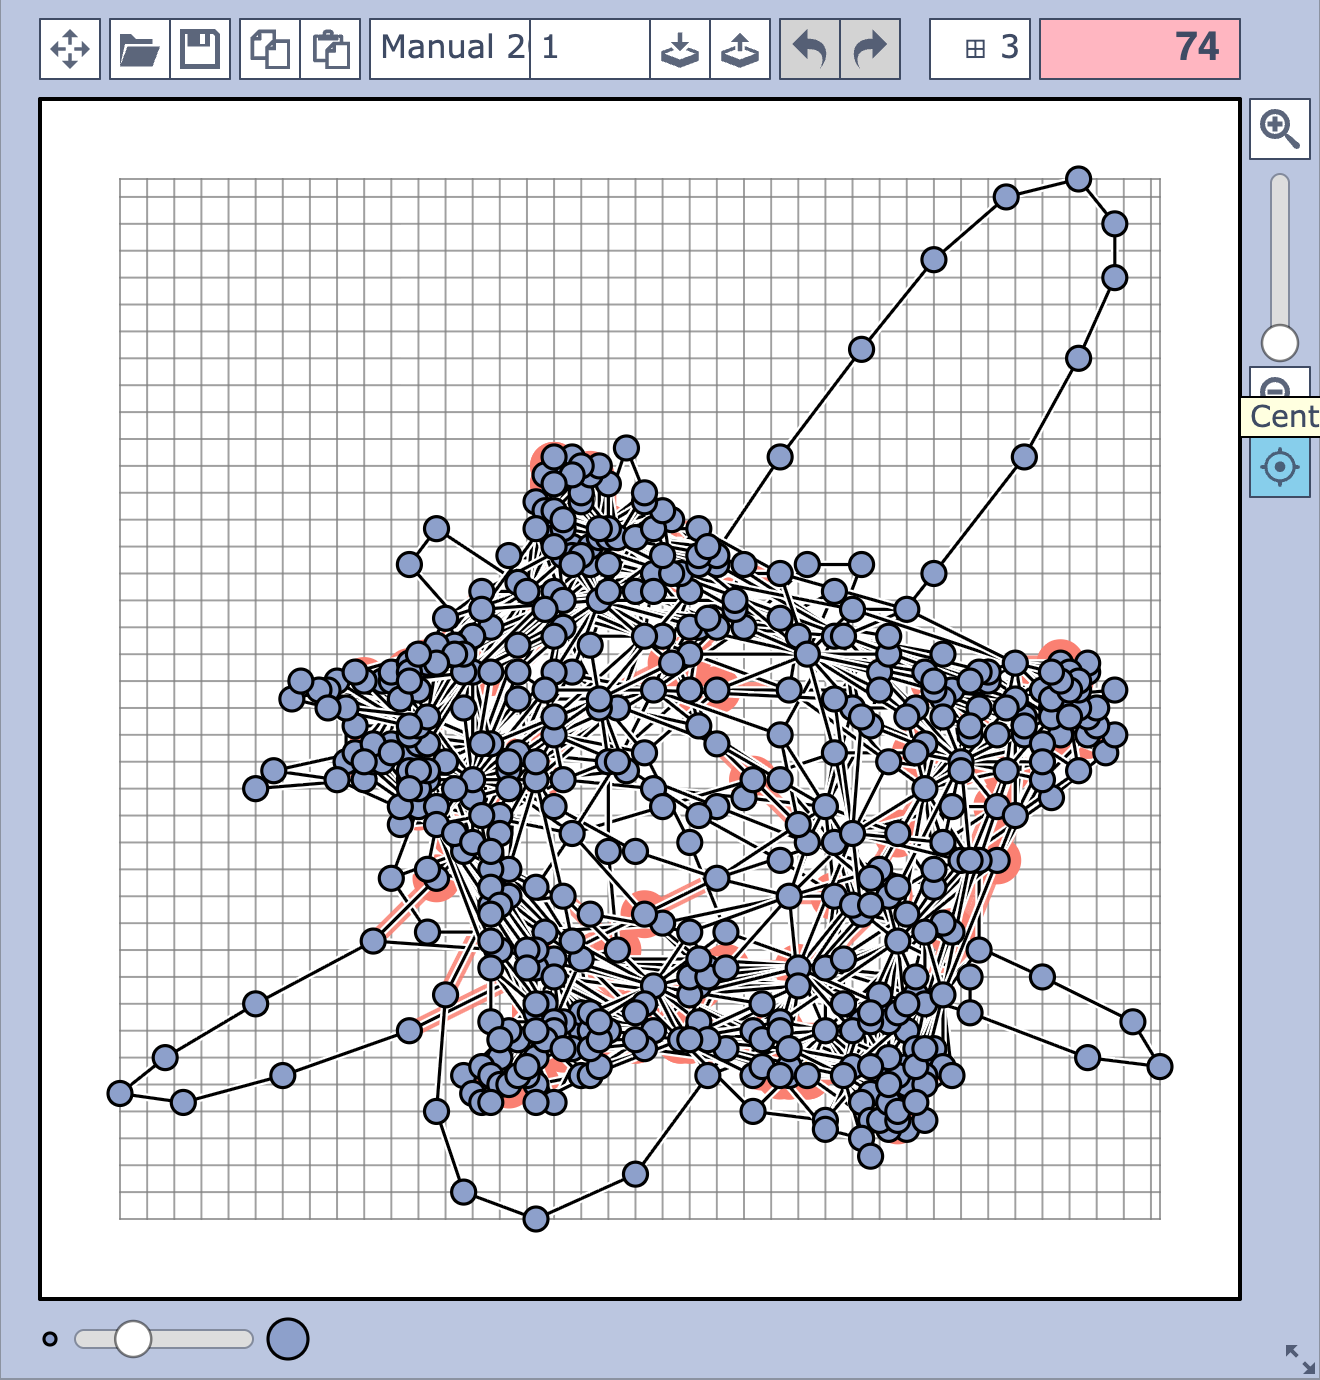
\includegraphics[width=\textwidth]{img/A7_1_stress.png}\\[2pt]
      \footnotesize\textbf{Stress Init}\\$k=74$
    \end{column}
    \begin{column}{0.23\textwidth}
      \centering
      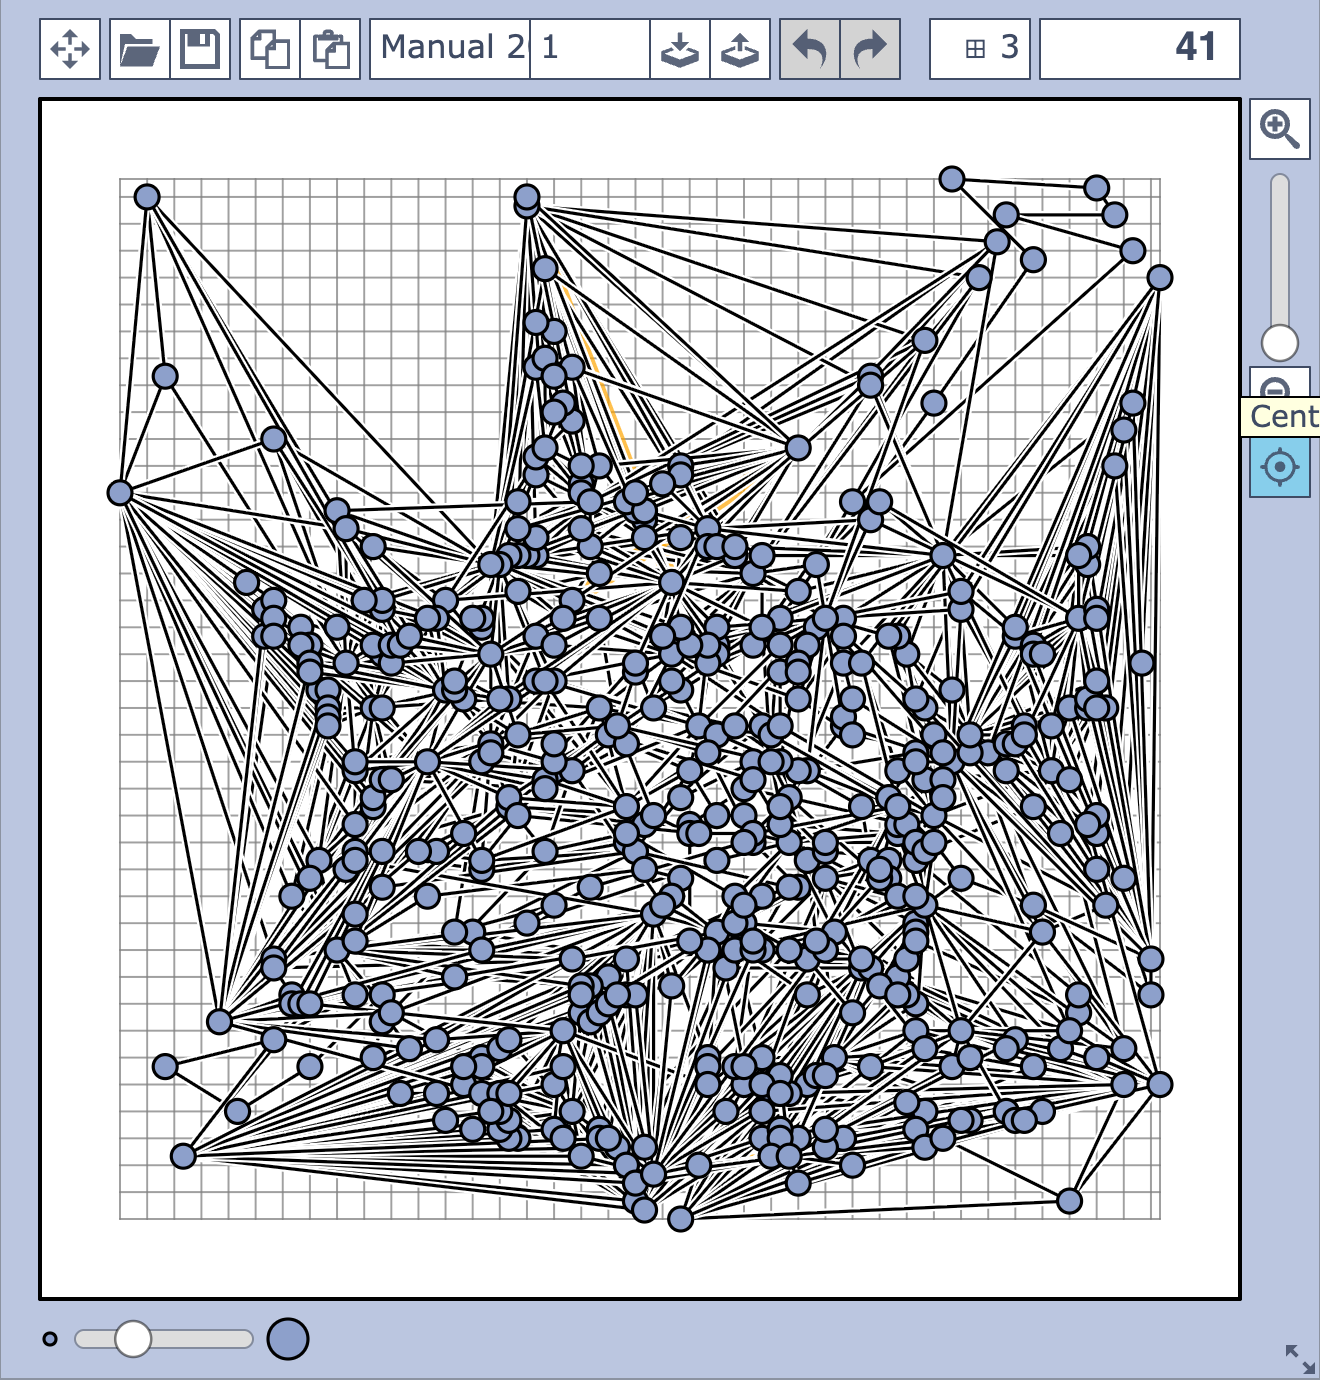
\includegraphics[width=\textwidth]{img/A7_2_phase1.png}\\[2pt]
      \footnotesize\textbf{Phase 1}\\$k=41$
    \end{column}
    \begin{column}{0.23\textwidth}
      \centering
      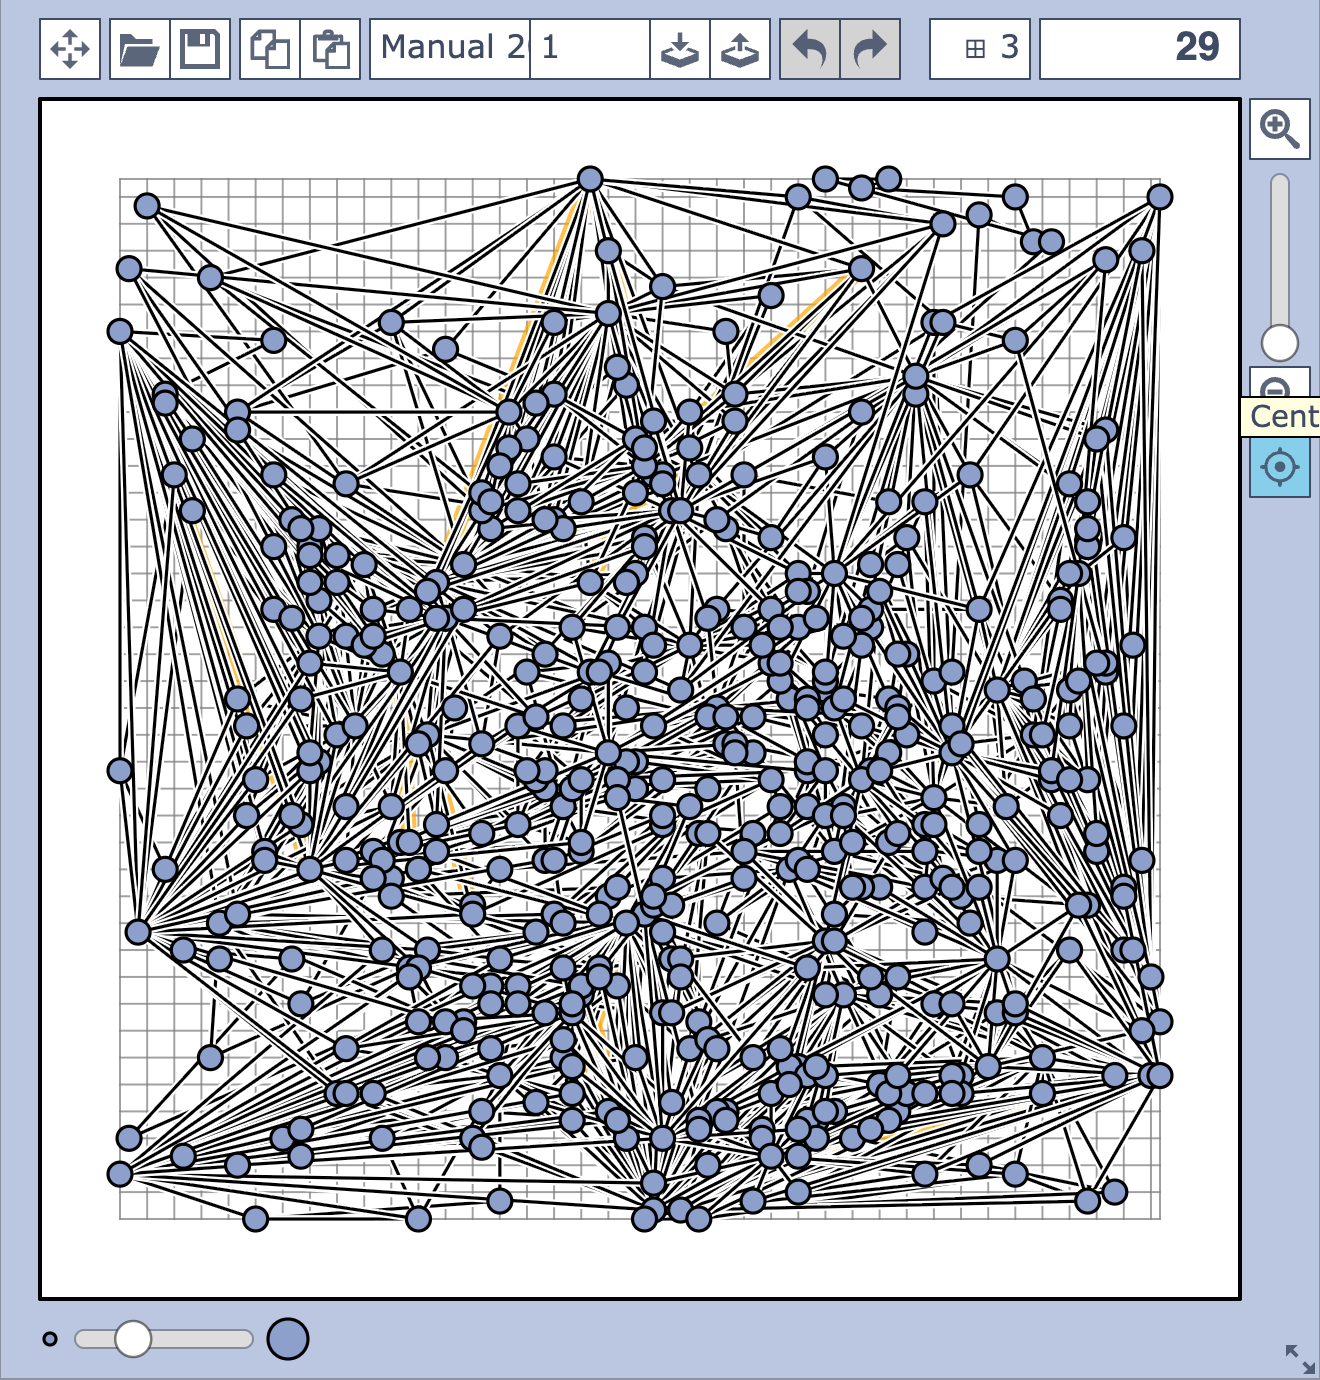
\includegraphics[width=\textwidth]{img/A7_3_phase2.png}\\[2pt]
      \footnotesize\textbf{Phase 2}\\$k=29$
    \end{column}
  \end{columns}
  \bigskip
  \centering
  \small Total: $858 \xrightarrow{\text{stress init}} 74 \xrightarrow{\text{Phase 1}} 41 \xrightarrow{\text{Phase 2}} \mathbf{29}$ \quad in \textbf{3\,min}
\end{frame}

\section{What We Built \& What We Found}

% ---------------------------------------------------------------
\begin{frame}{Correctness \& Throughput --- Making A8 Run At All}
  \textbf{Jun 5: Automatic-8 wrote no output.} The largest instance ($10\,466$ nodes
  in a tight $342{\times}294$ canvas) has vertices sitting on foreign edges, an
  invalid layout the solver must repair first. The old $O(n\cdot m)$ repair never
  converged, so the program exited without a file.
  \medskip

  Two fixes, both shipped in the final solver:
  \begin{itemize}
    \item \textbf{Grid-accelerated repair} --- A vertex grid shares the edge-grid
          geometry, so each vertex only checks nearby edges. Multi-pass relocation
          with expanding radius; A8 now repairs in \emph{seconds}.
    \item \textbf{\texttt{restoreBest} skip} --- Wave restarts recomputed \emph{all}
          crossings: \textbf{27\% of A8's phase-1 budget}. Skip it when the state
          already matches the best $\Rightarrow$ $342$k $\to$ $1.01$M moves
          (\textbf{$3\times$}).
  \end{itemize}
  \medskip
  \footnotesize A faster per-move overlap check and an LNS time-guard round out the
  throughput work.
\end{frame}

% ---------------------------------------------------------------
\begin{frame}{The Main Lever --- Stress Initialisation}
  \textbf{Reading the winners again} --- Our SA parameters already matched the winning
  paper \emph{exactly}. The real difference was their \emph{initialisation}: a
  force-directed layout (OGDF stress majorisation + FMMM).
  \medskip

  \textbf{Our method \texttt{sa-stress}} (\texttt{tools/stress\_init.py}) --- graphviz
  \texttt{sfdp}/\texttt{neato} $\to$ scale to canvas $\to$ integer grid snap $\to$
  spiral collision resolution, then the same two-phase SA on top. Same idea as OGDF,
  an off-the-shelf tool instead.
  \medskip

  \textbf{Pick the best candidate} --- Run the layout up to 8 times, estimate each
  one's crossing density from $200$k sampled edge pairs (a full count is $\sim$205M),
  hand the sparsest to SA.
\end{frame}

% ---------------------------------------------------------------
\begin{frame}{Stress Initialisation --- Why It Wins}
  \begin{center}
    \begin{tabular}{lrrr}
      \toprule
      full budget, 8 workers & A7 & A8 & A9 \\
      \midrule
      best before stress init   & 39 & 31 & 21 \\
      \textbf{with stress init}  & \textbf{28} & \textbf{7} & \textbf{10} \\
      \bottomrule
    \end{tabular}
  \end{center}
  \medskip
  \begin{itemize}
    \item \textbf{Not luck, reproducible} --- A \emph{single} 2.5-min run reaches
          $k=8\text{--}9$ on A8. The init alone starts SA at $k=24\text{--}27$, before
          a single move --- already past GD'25 winner ($15$). Best across runs: $\mathbf{7}$.
    \item \texttt{sfdp} beat \texttt{neato} everywhere; on $n>3000$ only \texttt{sfdp} runs.
    \item One exception: dense A6 resists \emph{any} init --- more on the final slide.
  \end{itemize}
\end{frame}

% ---------------------------------------------------------------
\begin{frame}{Phase 2 --- $k$-Critical Vertex Selection}
  \textbf{The observation} --- Phase 2 minimises the \emph{maximum} crossings on a
  single edge ($k$), but vertices were picked by their \emph{total} crossings ---
  effort spread everywhere except the bottleneck.
  \medskip

  \textbf{The change} --- Bias selection towards endpoints of edges within a band
  $\beta=2$ of the current $k$, with quadratic emphasis on proximity to $k$.
  \begin{itemize}
    \item \textbf{A/B (A7, 2\,min, same seeds):} $k=55/61$ with vs.\ $77/75$ without.
    \item \textbf{Hidden scaling bug, later fixed:} a fixed base mass made $\sim$97\%
          of A8's picks effectively uniform; scaling it to the critical mass restores
          $\sim$75\% critical picks at any $n$.
  \end{itemize}
\end{frame}

% ---------------------------------------------------------------

\section{Running the Whole Contest}

% ---------------------------------------------------------------
\begin{frame}{From One Graph to a Whole Contest}
  Our solver is strong \emph{per graph}. But the contest hands us \textbf{one
  wall-clock budget} (40--50\,min) to spend across \textbf{many graphs of unknown
  difficulty} --- and demands one valid layout for each, before time runs out.
  \medskip
  \begin{columns}[T]
    \begin{column}{0.5\textwidth}
      \textbf{Why a fixed split fails}
      \begin{itemize}
        \item Easy graphs reach $k{=}0$ in \emph{seconds} --- the rest of their
              slice is wasted.
        \item Hard graphs (dense, high $k$) are \emph{starved} --- they could use
              every banked second.
        \item Overrun by one move $\Rightarrow$ \textbf{missed submission}.
      \end{itemize}
    \end{column}
    \begin{column}{0.5\textwidth}
      \textbf{What the orchestrator must do}
      \begin{itemize}
        \item[\textcolor{accent}{\textbf{1}}] \textbf{Analyse} each graph up front.
        \item[\textcolor{accent}{\textbf{2}}] \textbf{Allocate} the budget where it
              still pays off.
        \item[\textcolor{accent}{\textbf{3}}] \textbf{Cooperate} across parallel workers.
        \item[\textcolor{accent}{\textbf{4}}] \textbf{Never overrun} the deadline.
        \item[\textcolor{accent}{\textbf{5}}] One best \emph{valid} layout per graph.
      \end{itemize}
    \end{column}
  \end{columns}
\end{frame}

% ---------------------------------------------------------------
\begin{frame}{Cooperative Workers: Half-Sharing}
  We ran $W$ workers per graph and asked: should they \emph{share} their best layout,
  and how does \emph{reheating} the temperature help? A controlled sweep on the live
  graphs (identical stress-inits, exact-verified $k$):
  \medskip
  \begin{columns}[T]
    \begin{column}{0.46\textwidth}
      \begin{itemize}
        \item \textbf{Reheat} (stagnation): neutral-to-negative $\Rightarrow$ left off.
        \item \textbf{Full sharing} --- all workers collapse onto one elite: helps
              \emph{high-}$k$ graphs, but \emph{hurts} low-$k$ ones (diversity dies).
        \item \textbf{Half-sharing} --- keep half exploring, let half intensify:
              \textcolor{teal}{\textbf{no-regret}}.
      \end{itemize}
      \medskip
      \footnotesize sum-$k$ over the hard graphs ($W{=}6$, 150\,s):
      \begin{center}\small
      \begin{tabular}{lc}
        \toprule
        independent (base)      & 618 \\
        full sharing            & 617 \\
        \textbf{half-sharing}   & \textbf{606} \\
        \bottomrule
      \end{tabular}
      \end{center}
    \end{column}
    \begin{column}{0.52\textwidth}
      \centering
      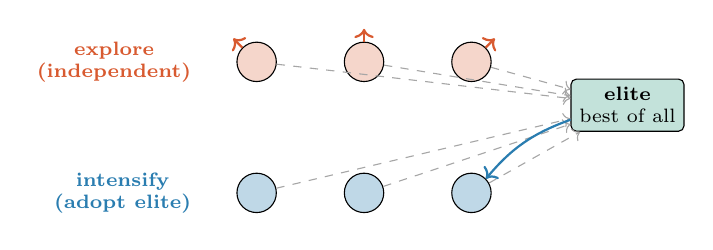
\begin{tikzpicture}[font=\scriptsize, node distance=0.42cm and 0.85cm,
          w/.style={draw, circle, minimum size=0.5cm, inner sep=0pt},
          box/.style={draw, rounded corners=2pt, align=center, inner sep=3pt,
                      minimum height=0.55cm}]
        % explorers (top row) with divergent arrows = diversity
        \node[w, fill=warm!25] (e1) {};
        \node[w, fill=warm!25, right=of e1] (e2) {};
        \node[w, fill=warm!25, right=of e2] (e3) {};
        \node[left=0.45cm of e1, text=warm, font=\bfseries\scriptsize, align=center]
             {explore\\(independent)};
        \draw[->, warm, thick] (e1) -- ++(135:0.42);
        \draw[->, warm, thick] (e2) -- ++(90:0.42);
        \draw[->, warm, thick] (e3) -- ++(45:0.42);
        % sharers (bottom row)
        \node[w, fill=accent!30, below=1.15cm of e1] (s1) {};
        \node[w, fill=accent!30, right=of s1] (s2) {};
        \node[w, fill=accent!30, right=of s2] (s3) {};
        \node[left=0.45cm of s1, text=accent, font=\bfseries\scriptsize, align=center]
             {intensify\\(adopt elite)};
        % elite (right, middle)
        \node[box, fill=teal!25, right=1.0cm of e3, yshift=-0.55cm] (el)
             {\textbf{elite}\\best of all};
        % every worker's best feeds the election
        \foreach \n in {e1,e2,e3,s1,s2,s3} \draw[->, gray!70, dashed] (\n) -- (el);
        % elite pulls the sharers next round
        \draw[->, accent, thick] (el) to[bend right=15] (s3);
      \end{tikzpicture}\\[2pt]
      \footnotesize Explorers keep feeding \emph{fresh} good layouts into the elite;
      sharers dig. Best-of-both, per graph.
    \end{column}
  \end{columns}
\end{frame}

% ---------------------------------------------------------------
\begin{frame}{The Orchestrator: Analyse $\to$ Explore $\to$ Reallocate}
  \centering
  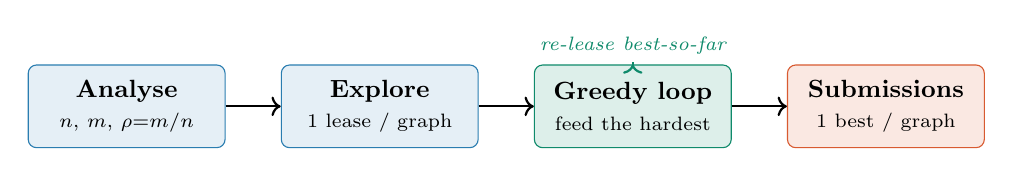
\begin{tikzpicture}[font=\small, node distance=0.7cm,
      stage/.style={draw, rounded corners=3pt, minimum height=1.05cm,
                    minimum width=2.5cm, align=center, fill=accent!12, draw=accent},
      lbl/.style={font=\scriptsize\itshape, text=muted}]
    \node[stage] (a) {\textbf{Analyse}\\{\scriptsize $n,\,m,\,\rho{=}m/n$}};
    \node[stage, right=of a] (e) {\textbf{Explore}\\{\scriptsize 1 lease / graph}};
    \node[stage, right=of e, fill=teal!14, draw=teal] (g)
         {\textbf{Greedy loop}\\{\scriptsize feed the hardest}};
    \node[stage, right=of g, fill=warm!14, draw=warm] (o)
         {\textbf{Submissions}\\{\scriptsize 1 best / graph}};
    \draw[->, thick] (a) -- (e);
    \draw[->, thick] (e) -- (g);
    \draw[->, thick] (g) -- (o);
    \draw[->, thick, teal] (g.north) to[out=120,in=60,looseness=4]
         node[above, lbl, text=teal]{re-lease best-so-far} (g.north);
  \end{tikzpicture}
  \medskip
  \begin{columns}[T]
    \begin{column}{0.54\textwidth}
      \textbf{Where does the next second go?}
      \[
        \text{priority}(g)=\frac{k_g \;\cdot\; \text{boost}_{\text{improving}}}
                                {\#\,\text{leases}_g}
      \]
      \begin{itemize}\footnotesize
        \item Worst graphs (high $k$) get the most --- but \emph{least-serviced
              rotates in}, so budget \emph{spreads} across all hard graphs.
        \item A graph that stops improving is \textbf{dropped}, banking its budget.
      \end{itemize}
    \end{column}
    \begin{column}{0.44\textwidth}
      \textbf{Every lease} runs the validated config:
      \begin{itemize}\footnotesize
        \item \texttt{sa-stress} (cold) $\to$ \texttt{sa-warm} continuation,
        \item $W$ workers with \textbf{half-sharing},
        \item warm-started from the graph's best-so-far.
      \end{itemize}
    \end{column}
  \end{columns}
\end{frame}

% ---------------------------------------------------------------
\begin{frame}{Deadline-Safe by Construction}
  \begin{columns}[T]
    \begin{column}{0.5\textwidth}
      \textbf{It cannot overrun.} A per-subprocess backstop clamps \emph{every} solver
      to a hard deadline that reserves time for the final verify + submission copy.
      A killed solver writes no file --- so the previous warm best is simply kept.
      \medskip

      \textbf{Fair spreading matters.} An early ``winner-take-all'' rule let one
      descent hog the budget; the least-serviced fix reclaimed the worst graph
      (\emph{same} 420\,s budget):
      \begin{center}\small
      \begin{tabular}{lcc}
        \toprule
                       & worst-$k$ & sum-$k$ \\
        \midrule
        winner-take-all & 283 & 666 \\
        \textbf{fair spread} & \textbf{252} & \textbf{639} \\
        \bottomrule
      \end{tabular}
      \end{center}
    \end{column}
    \begin{column}{0.47\textwidth}
      \centering
      \textbf{Validation --- 9 graphs, one budget}
      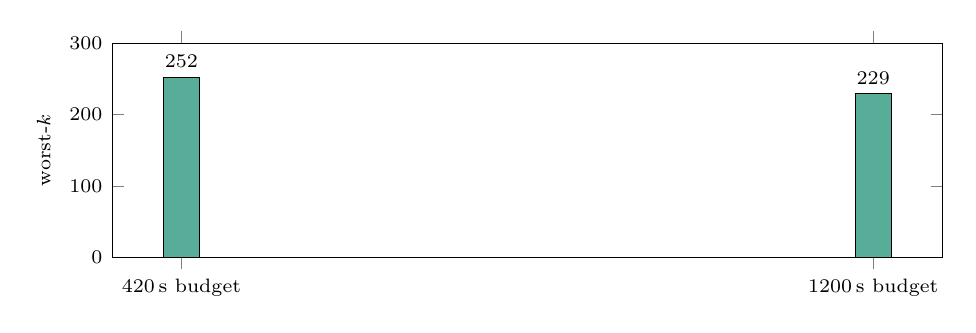
\begin{tikzpicture}
        \begin{axis}[width=\linewidth, height=4.3cm,
            ybar, bar width=13pt,
            symbolic x coords={420s,1200s},
            xtick=data, ymin=0, ymax=300,
            ylabel={worst-$k$}, ylabel style={font=\scriptsize},
            xticklabels={420\,s budget,1200\,s budget},
            nodes near coords, every node near coord/.append style={font=\scriptsize},
            tick label style={font=\scriptsize}]
          \addplot[fill=teal!70] coordinates {(420s,252) (1200s,229)};
        \end{axis}
      \end{tikzpicture}\\[-2pt]
      \footnotesize
      420\,s budget $\to$ finished in \textbf{381\,s}, \textbf{all 9 valid}.\\
      More budget $\to$ lower $k$; the hard graphs soak up the banked time.
    \end{column}
  \end{columns}
\end{frame}

% ---------------------------------------------------------------
\begin{frame}{One Folder, One Click}
  Wired straight into the dashboard --- a \textbf{Batch / Orchestrator} toggle in the
  run-control panel:
  \medskip
  \centering
  \begin{tikzpicture}[font=\small, node distance=0.55cm,
      step/.style={draw, rounded corners=3pt, minimum height=0.95cm,
                   minimum width=2.35cm, align=center}]
    \node[step, fill=muted!15] (f) {\textbf{Pick folder}\\{\scriptsize of graphs}};
    \node[step, fill=accent!15, right=of f] (s) {\textbf{Scan}\\{\scriptsize preview graphs}};
    \node[step, fill=teal!18, right=of s] (r) {\textbf{Scan \& Run}\\{\scriptsize auto-start}};
    \node[step, fill=warm!15, right=of r] (m) {\textbf{Live monitor}\\{\scriptsize log + $k$ table}};
    \draw[->, thick] (f) -- (s);
    \draw[->, thick] (s) -- (r);
    \draw[->, thick] (r) -- (m);
  \end{tikzpicture}
  \medskip
  \begin{columns}[T]
    \begin{column}{0.5\textwidth}
      \begin{itemize}
        \item Type the graph folder $\to$ \texttt{Scan} lists every valid graph found.
        \item \texttt{Scan \& Run} launches the orchestrator on that folder --- no
              other setup.
      \end{itemize}
    \end{column}
    \begin{column}{0.5\textwidth}
      \begin{itemize}
        \item Live log + per-graph \texttt{k\,/\,leases\,/\,valid} stream while it runs.
        \item Submissions land in \texttt{submission/}, keeping the \emph{original}
              file names.
      \end{itemize}
    \end{column}
  \end{columns}
  \medskip
  \centering
  \small\textcolor{teal}{\textbf{Analyse $\to$ allocate $\to$ half-share $\to$ submit --- inside the budget, hands-off.}}
\end{frame}

\section{Results \& Lessons}

\begin{frame}{Final Results: All Nine Instances}
  Best validated $k$ per instance (accumulated over our runs), against last year's
  live leaderboard and the GD'25 winning team:
  \begin{center}
    \footnotesize
    \begin{tabular}{lrrll}
      \toprule
      \textbf{Graph} & \textbf{Ours} & \textbf{Method} & \textbf{GD'25 winner} \\
      \midrule
      Automatic-1 & 9   & \texttt{sa}        & 9   \\
      Automatic-2 & 3   & \texttt{sa}        & 3   \\
      Automatic-3 & 35  & \texttt{sa}        & 34   \\
      Automatic-4 & 6   & \texttt{ils}       & 6   \\
      Automatic-5 & 75  & \texttt{staged}    & 76   \\
      Automatic-6 & 624 & \texttt{sa}        & 568 (49\,min) \\
      Automatic-7 & \textbf{28}  & \texttt{sa-stress}   & 31   \\
      Automatic-8 & \textbf{6}   & \texttt{sa-stress}   & 15   \\
      Automatic-9 & \textbf{10}  & \texttt{sa-stress}   & 12   \\
      \bottomrule
    \end{tabular}
  \end{center}
  \smallskip
  \begin{itemize}
    \item \textbf{Ahead of the winning team on A7, A8, A9} (A8: $15 \to 6$);
          A6 is the one open front.
  \end{itemize}
\end{frame}

\begin{frame}{Automatic-8: What Each Improvement Bought}
  \centering
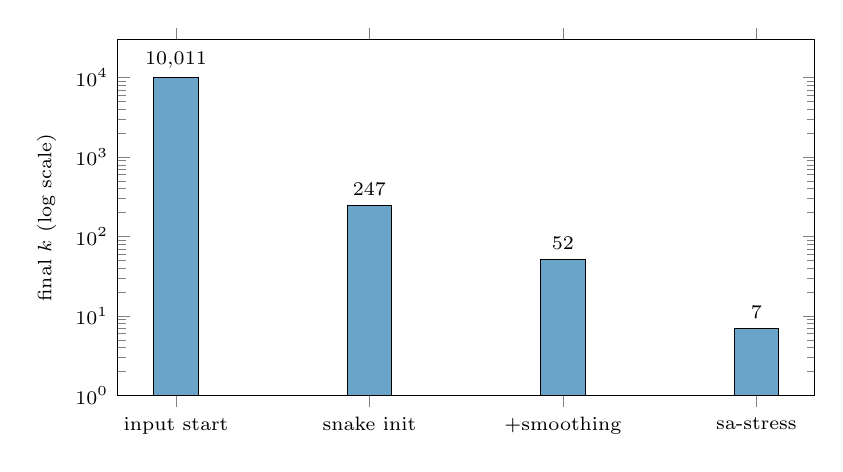
\begin{tikzpicture}
    \begin{axis}[width=0.86\linewidth,height=6.1cm,
        ybar, bar width=16pt,
        symbolic x coords={input start,snake init,+smoothing,sa-stress},
        xtick=data, ymode=log, log origin=infty,
        ymin=1, ymax=30000,
        ylabel={final $k$ (log scale)},
        point meta=rawy,
        nodes near coords={\pgfmathprintnumber[fixed,precision=0]{\pgfplotspointmeta}},
        every node near coord/.append style={font=\scriptsize},
        tick label style={font=\scriptsize},label style={font=\scriptsize}]
      \addplot[fill=accent!70] coordinates
        {(input start,10011) (snake init,247) (+smoothing,52) (sa-stress,7)};
    \end{axis}
  \end{tikzpicture}

  \smallskip
  Setup: $\sim$12\,min $\to$ $\sim$8\,s. Validity: \emph{none} $\to$ exact-verified on all graphs.
\end{frame}


\begin{frame}{What Remains \& Takeaway}

  \textbf{If you remember one thing:}
  \begin{center}
    \emph{We took the winning team's solver design, made it correct on the hardest input,
    3$\times$ faster in the move loop on that instance, and gave it a better starting
    point ---\\
    and that was enough to beat the winner's published results on a third of the instances.}
  \end{center}
  \medskip
  \begin{itemize}
    \item Code, pipeline, dashboard and all experiment logs:
          \texttt{github.com/kahlery/graph-contest}
  \end{itemize}
\end{frame}


\end{document}
